\documentclass[10pt, a4paper]{article}

\usepackage[english]{babel}
\usepackage{circuitikz}
\usepackage{float}
\usepackage{enumitem}
\usepackage{graphicx}
\usepackage{subcaption}
\usepackage{amsmath}
\usepackage{siunitx}

% Define environment for question
% Set counter for questions
\newcounter{qcounter}
% Start at value one
\setcounter{qcounter}{1}
 % Define the command
\newcommand{\q}[2]{
    \begin{description}
        \item[Q~\arabic{qcounter}\refstepcounter{qcounter}:] \textbf{#1}
        \item[A:] {#2}
    \end{description}
}

\begin{document}
\begin{titlepage}
    \centering
    {\scshape\LARGE Robust Mechatronics, MF2042 \par}
    \vspace{1cm}
    {\scshape\large Solutions to Exam April 2015 \par}
    \vfill
    Andreas Froderberg
\end{titlepage}
% Part A 
{\centering \scshape \LARGE\underline{Part A} \par}
\q{If you have a series pass voltage regulator (linear, like the 7805), why is
    that givin less noise than a switched regulator?}
  {The current in a linear regulator is always on and the transforming (always
down) is done by "burning" surplus voltage. In contrast, the switching regulator
regulates the voltage by switching parts of the regulating circuit on and off.
Quickly changing current means EMI and the "hot loop" (switching part of
circuit) cand even act as an antenna.}
\q{What differences are there for a ground wire compared to a ground plane?}
{In a ground plane, the return signals (at higher frequencies, kHz) are able to
    trace back under the original signal, giving lower impedance than in a
ground wire.}
\q{Sketch a step up (Boost) converter. Show the current path in both on and off.
Is there part of it that is more sensitive to radiated emissions and why?}
{ What if i add some text first?
    % Boost converter
    \begin{figure}[H]
        \centering
        \begin{circuitikz} \draw
                (0,4) node[left] {$V_{in}$}
                to[L=L, o-*] (3,4)
                to[zD*, -o] (6,4)
                to[C=C] (6,0)
                node[ground] {} 
            (3,0) node[ground] {}
                to[switch] (3,4)
            (8, 4) node[right] {$V_{out}$}
                to[short, o-] (6,4)
                ;
        \end{circuitikz}
    \end{figure}
    When the switch is off, the current is flowing through the coil and into the
    load through the diode with the capacitance as filter. When the switch is on, the current is
    going through the coil via the switch into ground. The hot loop (radiating
    part) is through the coil and switch. This is where the current differences
    are largest at the switching.
}
\q{You have an analog sensor signal that you should sample with your
    microcontroller. When should you apply (also discribe shortly why)\ldots
    \begin{enumerate}[label=(\alph*)]
        \item \ldots an analog filter?
        \item \ldots a digital filter?
    \end{enumerate}
}
{\begin{enumerate}[label=(\alph*)]
        \item An analog filter should be used before the ADC to avoid aliasing.
            The cutoff frequency should be no lower than the Nyquist frequency,
            $\omega_s/2$, where $\omega_s$ is the sampling frequency.
        \item A digital filter is well suited for more advanced filters such as
            higher order filters and filters of Butterworth and Chebyshev
            type. 
    \end{enumerate}
}
\q{If you have an electric vehicle and battery voltage 600 V, you have to
    isolate the low voltage (48 V) from the high voltage. How do you do that for
    both digital and analog signals?
}
{
    One solution is to use an isolated DC-DC converter which galvanically
    isolates the two voltages. This is expensive though. One way of separating
    digital and analog signals is the use of partitioning which means that the
    PCB has dedicated parts for analog and digital and a zone between where no
    signal paths are allowed.
}
\q{
    A sensor is connected to an amplifier either by straight wires or a twisted
    pair, see picture. What will be the difference with respect to radiated
    susceptability if you put these two setups into an electromagnetic field?
    Why will there be a difference?
    \begin{figure}[H]
        \centering
        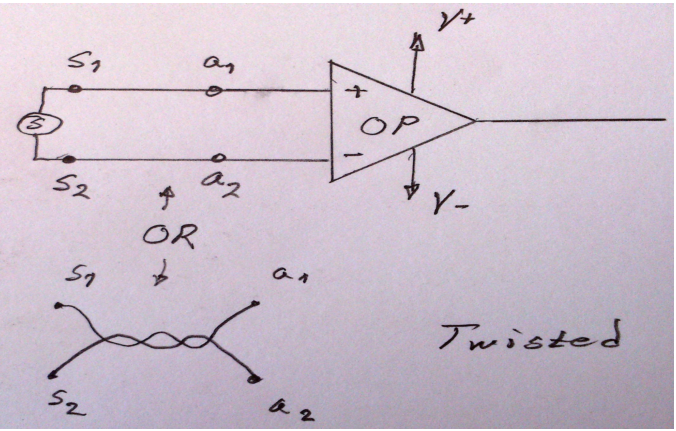
\includegraphics[width=0.7\linewidth]{twisted.png}
    \end{figure}
}
{
    If put in an electromagnetic field, the cabling becomes a loop antenna.
    The direction of the current is dependant on the direction of the magnetic
    field. In the untwisted pair, interference currents will start flowing
    causing interference. In the twisted pair,  the polarity is switched at
    every intersection. This will cause alternating currents in every twist,
    canceling each other out (mostly).
    \begin{figure}[H]
        \centering
        \begin{subfigure}[t]{0.4\textwidth}
            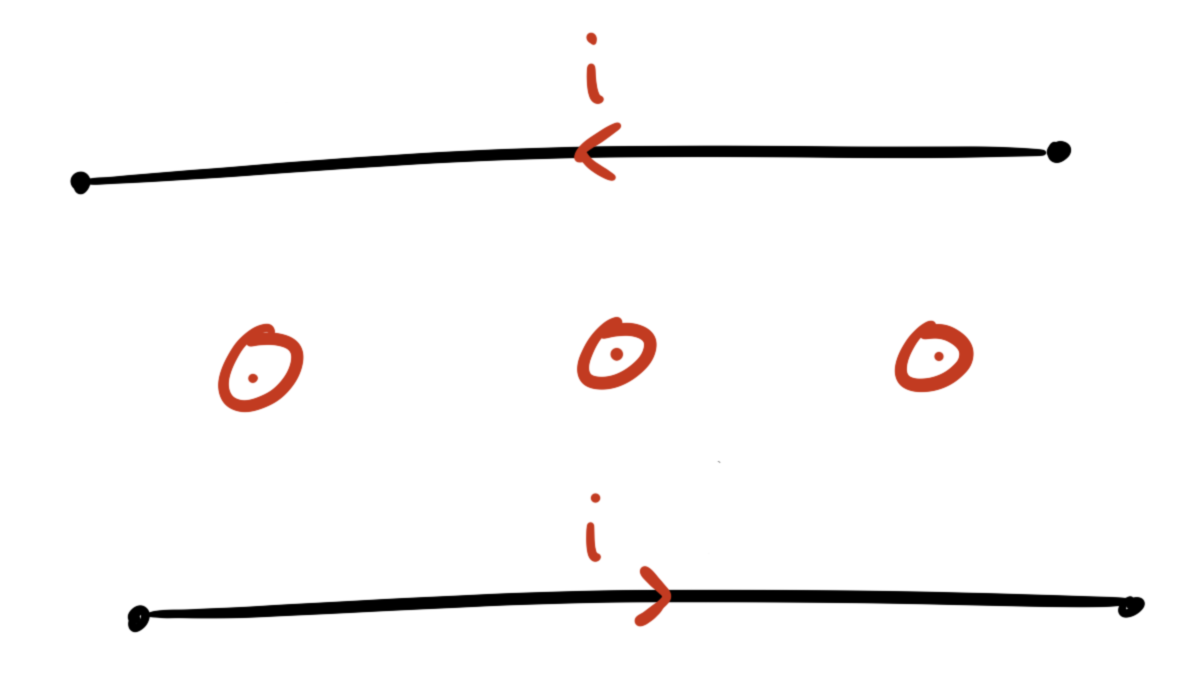
\includegraphics[width=\textwidth]{untwisted.png}
        \end{subfigure}
        \begin{subfigure}[t]{0.4\textwidth}
            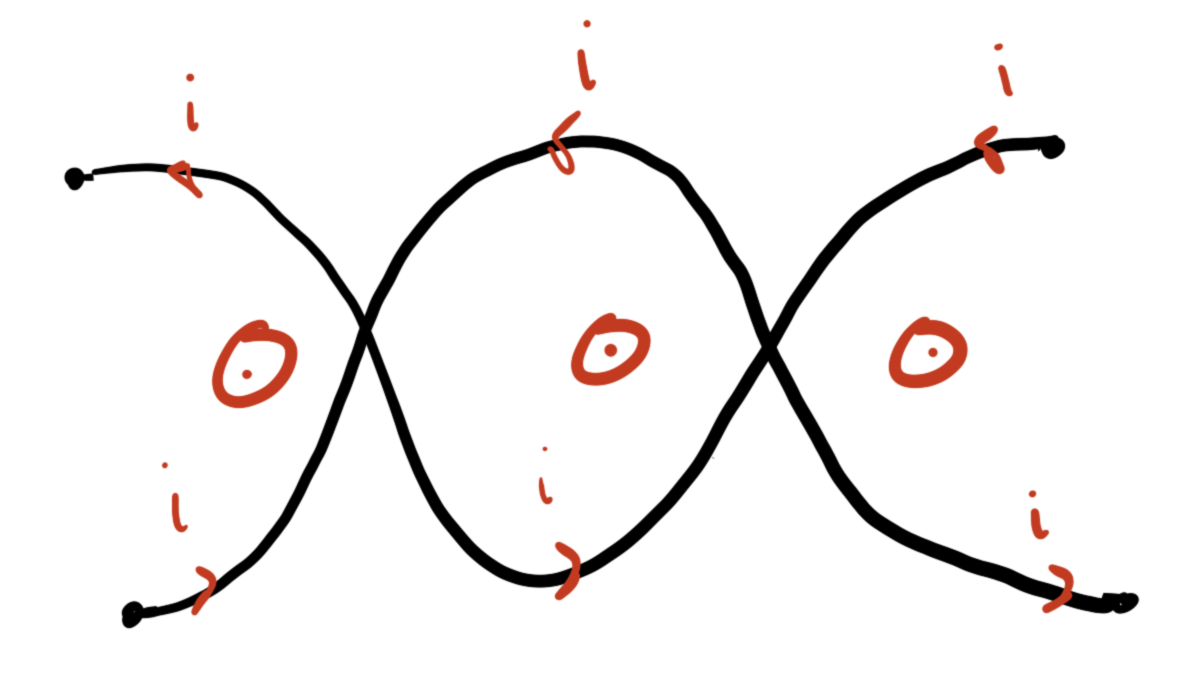
\includegraphics[width=\textwidth]{twisted1.png}
        \end{subfigure}
    \end{figure}
}
\q
{
    You have a common mode voltage of 8V into an instrumentation amplifier and
    1V of signal. What voltage can you measeure on the two pins? (It does not
    matter which pin the voltage is measured on)
}
{
    Common mode voltage is calculated 
    \begin{equation*}
        U_{CM} = \frac{U_1 + U_2} {2}
    \end{equation*}
    If $U_{CM}=8V$ and $U_1 - U_2 = 1V$, then
    \begin{equation*}
        U_{1} = U_{CM} - 0.5 = 8 - 0.5 = 7.5\si{\volt} \text{ and } U_2 =
        8.5\si{\volt}.
    \end{equation*}
}
\clearpage
% Part B 
{\centering \scshape \LARGE\underline{Part B} \par}

\clearpage
\end{document}
